\documentclass[11pt]{article}
% Use wide margins, but not quite so wide as fullpage.sty
\marginparwidth 0.5in 
\oddsidemargin 0.25in 
\evensidemargin 0.25in 
\marginparsep 0.25in
\topmargin 0.25in 
\textwidth 6in \textheight 8 in
% That's about enough definitions

\usepackage{setspace}
\usepackage{url}
\usepackage{amsmath}
\usepackage{graphicx}

\begin{document}
\author{Mark Gius\vspace{10pt} \\
        Advisor: Dr. Zo\"e Wood
        }
\title{Senior Project: AutoRPG}
\maketitle

\begin{abstract}
Most video games on the market today are geared towards players with fast reflexes and favor quick action over careful planning. This trend has particularly affected the Console Role Playing Game.  Where in the past the pace of the game afforded time to choose an action and select it, newer games progress at a breakneck pace, leading to less direct player interaction and more scripted actions.

I implemented a 2D game in the style of Super Nintendo RPGs using PyGame, a Python game development framework.  The game includes a simple frontend ``overworld'' that allows the player to move around and initiate battles with enemy characters. PyGame's builtin collision detection modules are used to prevent characters from walking through walls or each other.  In addition, a ``battle'' screen highlights the effects of the player character doing battle with various NPCs. The ``battle'' system is implemented such that user control over characters is driven entirely by pre-defined character behavior that the user will control.

\end{abstract}

\doublespacing
\section{Introduction}

Most video games on the market today are geared towards players with fast reflexes and favor quick action over careful planning. This trend has particularly affected the Console Role Playing Game.  Where in the past the pace of the game afforded time to choose an action and select it, newer games progress at a breakneck pace, leading to less direct player interaction and more scripted actions.  One such game, Final Fantasy XII, allowed the player to provide sets of actions for their characters to perform automatically in battle in addition to manually entered actions. \cite{Gambits} This preserved a significant amount of tactical planning in the game. A well-designed set of actions could often make the difference between victory and defeat.

A game that only allowed battle actions through pre-defined character tactics would force the player to think deeply about their opponents and characters in order to develop a winning strategy. 

To achieve this goal, a simple game was developed that features a battle system that only allows player interaction via predefined sets of rules that are evaluated each round in order to select an action.  These rules consist of a Condition which must be present in order to perform an associated Action.  For example, a rule might direct a character to focus their efforts on the enemy with the lowest defense. The same system drives enemy combatant behavior, resulting in enemies whose behavior can be analyzed and appropriate strategies formed to triumph over them.

In addition to the backend that drives combat, a simple ``overworld'' screen was developed that features block based movement and simple sprites in the style of older RPG games.  The overworld screen also presents character movement using simple animations as the characer moves about the screen.  

A secondary goal of the project was to provide the ability to quickly and painlessly add new game assets in a human readable way.  Many elements of the game are stored as human readable and editable text files on the disk.  These game assets include character and monster definitions, equipment definitions and world definitions.

\section{Previous Work/Related Work}

There are several other games that feature similar gameplay mechanics.  

\begin{description}
\item[RoboCode \cite{RoboCode}] \hfill \\
      ``Robocode is a programming game, where the goal is to develop a robot battle tank to battle against other tanks in Java or .NET.'' Robocode contains a similar ``AI'' approach to player interaction, but requires the user to create their AI in a supported programming language.  This limits the potential audience to programmers and those willing to learn.  Ideally non-programmers would be able to play the game as well.

\item[Final Fantasy XII \cite{Gambits}] \hfill \\
      Final Fantasy XII is the primarily influence for AutoRPG. Final Fantasy XII allows for the player to override the pre-programmed strategies at any time.  This allows a sufficiently fast player to react to battle events as they occur rather than predicting them ahead of time.  Ideally players would not be rewarded to quick reflexes but for thinking ahead and planning out their strategy in advance.

\end{description}

\section{Implementation}

A simple prototype game was developed in Python using the PyGame game development framework.  The project can be largely split into two sections: the frontend, or ``Graphical'', components and the backend code that drives the battle system.  

\subsection{Frontend}

The frontend largely serves to display the information for the battle.  It serves a secondary purpose of allowing future development to take the project from proof of concept to full fledged game if future developers so desired.

\subsubsection{Block Based Movement}

In most SNES era RPG games, player characters moved about the overworld in discrete steps as though the world was divided into a grid.  A single press of any direction would cause movement until the player was fully contained in the next block created by the grid.  I wanted to recreate this behavior for the simple overworld screen.

\begin{figure}[h!]
\begin{center}
\leavevmode
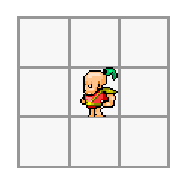
\includegraphics[]{images/overworld_blocks}
\end{center}
\caption{Character in the middle of a grid.  Movement cannot stop unless 
         a character is entirely contained in a single grid box.}
\end{figure}


The block based movement algorithm implemented has the following characteristics:
\begin{description}
   \item[Characters must move in discrete blocks] \hfill \\
   Movement must begin and end on specific points on a grid.  Characters cannot stop between these points and cannot change direction except on these specific points. 
   \item[The current direction takes precedence] \hfill \\
   So long as the direction key corresponding to the current direction continues to be held down, the player will continue walking that direction.  The addition of additional direction keys has no effect on the current directions.
   \item[The order that directions are pressed matters] \hfill \\
   If several directions are pressed at the same time, the first one pressed takes precedence.  A player that holds down right, then presses and holds up followed by down, will find their character moving up when right is released.
\end{description}

This behavior is achieved using a bitset and a queue.  

PyGame contains an event system for tracking input events from a keyboard, mouse or joystick.  A PyGame library call provides the caller with a queue of events that have occurred since the last call to the event system.  Keyboard presses are processed as events to be handled by the game code.  For every keypress, PyGame generates two events: one when the key is depressed, and one when it is released.  Because PyGame does not track the current state of input devices itself, we must keep track of the current state of the keyboard ourselves.  This is where the bitset is used.  Each direction is assigned a value that can be expressed as a power of two. These values can be stored by using bitwise operators.  For example:

\begin{align*}
Left = 00000001 \\ 
Right = 00000100 \\
Left \land Right = 00000101 \\
Left \land Right \land \neg Right = 00000001 \\
None = 00000000
\end{align*}

When keys are depressed, the appropriate number is bitwise ANDed into the bitset.  On key release the inverse of the appropriate number is bitwise ANDed, removing that bit from the set.  By querying the bitset, the set of depressed keys can be returned.

The bitset is useful for determining which keys are currently depressed, but it does not provide any information about the order in which keys were depressed.  To keep track of the ordering of keypresses, The set of keypresses are also recorded in a queue, to preserve the order of the keypresses.  At each frame update, the character sprite is animated and moved around the screen based on its current movement direction.  

When the character reaches a grid intersection point, a new direction must be chosen.  The current direction is used to determine if that key is still depressed. If so, the character continues moving in the same direction.  If not, the queue of directions is used. Each direction in the queue is compared against the current set of depressed keys.  When a direction is found that is still depressed, the character moves in that direction.  The queue is emptied when the character has stopped and all keys have been released.

The implementation for block based movement can be found in \texttt{character/character.py} in the \texttt{Character} and \texttt{PlayerCharacter} classes.

\subsubsection{Animations}

PyGame has no native support for animated characters, so I had to develop my own.  Animations are implemented as a circularly linked list, where each element in the list represents a single frame of the animation.  The linked list itself has no notion of display frames vs animations frames.  It simply responds to requests for ``next frame in the animation.''  Python has a native implementation of a circularly linked list\footnote{The \texttt{cycle} class in the \texttt{itertools} module}, but it lacks the important ability to reset the list back to the beginning of the cycle.  At this time, most of the animations are simple two-frame walking animations, but I wanted to support more complex animations as well.  In order to support longer animations, the frontend code needed to be able to reset the animation back to the ``start'' to ensure that the animation will begin where expected.  Due to this weakness, I reimplemented the native Python cycle based upon their specification in the Python documentation \cite{PythonCycle} and added a reset function to restore the cycle to it's original state. 

Currently all animations are progressed at a rate of three frames per second.  This framerate could be easily modified or abstracted out so that different animations progress at different rates.  This would require a certain amount of overhead to implement an Animation Class that would contain information about the frames of the animation and the rate at which frames should be cycled. 

The implementation for the resettable cycle can be found in \texttt{shared/cycle.py} in the \texttt{Cycle} class. 

\subsection{Battle Backend}

Underneath the visual layer is a simple turn based RPG system.  Battleable characters have attributes such as hit points and equipment that define how they fare in battle.  Characters can interact with each other using their equipment or magic spells.  Characters also contain attributes that help the GUI frontend, such as animation and location data.

\subsubsection{Data Loading}

One of the secondary goals of the project was to be able to quickly add game assets in a human readable way.  In accordance with this goal, almost every aspect of a character can be expressed and stored as human readable json objects on the file system.  Several other container formats were considered, including XML and Python's native ``configuration'' format.  JSON \cite{JSON} was chosen primarily for its simplicity and human readability.  It is much easier to read and write by hand than XML while still being able to contain the same information.  A side benefit of using JSON is its similarity to Python dictionary notation.  A JSON object can be interpreted wihout modification by the Python interpreter as a Python dictionary object, making the syntax even more friendly for Python developers hoping to extend the project.  Python also features a simple JSON library that simplifies reading and writing to and from JSON data.

All loading of configurable data, like Characters and their Equipment, is done via a set of load functions that can be found in the \texttt{shared.load} module. This module centralizes disk read activity so that the code in other modules does not need to have awareness of where files are located or the format of the stored data.  Because all code in the project expects that these load functions return dictionary values the underlying data type can be changed in the future if desired, so long as the load functions continue to return dictionaries.

After the data is read off of the disk, a particular class will use the information contained within to populate its attributes for use within the game.  For example, the following code is executed every time a player is instantiated:

\singlespacing
\samepage{
\begin{verbatim}
def load_player(name, center=None):
   jsonData = load_character_data(name)
   return globals()[jsonData['charactertype']](jsonData, center)

class BattleablePlayerCharacter(PlayerCharacter, BattleableCharacter):
   def __init__(self, jsonData, center=None):
      displayname = jsonData['charactername']
      spritename = jsonData['spritename']

      PlayerCharacter.__init__(self, spritename, displayname, center)
      BattleableCharacter.__init__(self, jsonData)
\end{verbatim}
}
\doublespacing

Not all aspects of this code will be explained in full.  Interested parties may find the official Python Documentation \cite{PyDocs} very helpful, especially the sections on Python classes.

Code wishing to load a character from disk would call the load\_player function with a string argument containing the name of the character to load.  load\_player then loads the JSON data corresponding to that character from the disk.  There can be multiple types of players, ranging from Non Player Characters to Groups of characters represented by a single in-game sprite.  The second line of load\_player should be broken down a little bit.  

Python contains a builin functions,\texttt{globals()}, that returns a dictionary of the current scope's global variables. Contained in that dictionary, among other things, is a mapping from the string ``BattleablePlayerCharacter'' to the Class object for the BattleablePlayerCharacter class.  The player we have just loaded happens to be a BattleablePlayerCharacter, so the ``charactertype'' attribute in the JSON data contains the string ``BattleablePlayerCharacter.'' Once the Class object has been retrieved, we can call the constructor for that class on it, passing in the retrieved JSON data and an optional location in the world to place the character. 

Within BattleablePlayerCharacter, two attributes are retrieved from the JSON dictionary, and then the initialization function for the two classes that BattleablePlayerCharacter inherits from are executed.  PlayerCharacter primarily sets up display attributes such as the animation frames and sets up keyboard input rules for that character.  BattleableCharacter initializes all of the attributes used by the battle system, such as equipment and hit points, as we can see from the BattleableCharacter code:

\singlespacing
\samepage{
\begin{verbatim}
# partial class implementation
class BattleableCharacter(Character):
   def __init__(self, jsonData):
      ''' Does not call Character.__init__ intentionally '''
      self.charactername = jsonData['charactername']

      self.maxhp = jsonData['maxhp']
      self.curhp = jsonData['curhp'] if 'curhp' in jsonData else self.maxhp

      self.maxmp = jsonData['maxmp']
      self.curmp = jsonData['curmp'] if 'curmp' in jsonData else self.maxmp

      self.speed = jsonData['speed']
      
      self.weapon = equipment.Weapon.load(jsonData['weapon'])
      self.armor = equipment.Armor.load(jsonData['armor'])
\end{verbatim}
}
\doublespacing

The instantiated BattleablePlayerCharacter object is now ready to be used in battle and controlled by the player in the overworld.

Code for the \texttt{PlayerCharacter} and \texttt{BattleableCharacter} classes can be found in the \texttt{character.character} module.

\subsubsection{Strategems}

The battle action in AutoRPG is controlled by a given character's Strategy.  A Strategy is composed of one or more Strategems.  A Strategem is composed of a single \emph{Condition} and \emph{Action}.

Most of the code related to the Strategem system can be found in the \texttt{strategem} module.  The driver for the Strategem system can be found in the \texttt{environment.battlescreen} module, in the \texttt{BattleField} class's \texttt{update} method.

\paragraph{Conditions} \hfill % force header-ish formatting

\emph{Conditions} define under what circumstances an associated \emph{Action} should be executed. A \emph{Condition} definition is relatively simple.  

\singlespacing
\samepage{
\begin{verbatim}
class EnemyHealthBelow(Condition):
   def __init__(self, extradata):
      self.threshold = extradata['hpThreshold']

   def checkCondition(self, attacker, defenders):
      for defender in defenders:
         if defender.hp < self.threshold:
            return defender

      return None
\end{verbatim}
}
\doublespacing

Each condition contains a single method, \texttt{checkCondition}, that returns either a character to be targeted or a \texttt{None} object, signifying that no target was acceptable and the next Strategy should be evaluated.

This \emph{Condition} will trigger when one of the opponents' health reserves has dropped below a particular point.  The condition iterates through each potential defender (provided by the Strategem driver) until it finds an attacker that meets the threshold defined by the attacker's Strategem configuration.

\paragraph{Actions} \hfill % force header-ish formatting

Actions are, well, actions that a character can perform in battle.  Example actions include attacking with an equipped weapon or casting a magic spell.  An Action's behavior is defined by a Python class that corresponds to a particular action that can be performed.

An example \emph{Action} can be seen below:

\singlespacing
\samepage{
\begin{verbatim}
class CastSpell(Action):
   def __init__(self, extradata):
      self.spellname = extradata['spellname']
      self.spell = None
      self.lastAttacker = None

   def canDoAction(self, attacker, defender):
      if self.lastAttacker is not attacker or self.spell is None:
         self.spell = None
         for spell in attacker.spellbook:
            if spell.name == self.spellname:
               self.spell = spell
               break
         if self.spell is None:
            return False
      return attacker.curmp >= self.spell.mpcost

   def doAction(self, attacker, defender):
      damage = self.spell.getDamage()
      if element.isWeak(self.spell.elem, defender.armor.elem):
         damage *= 2
      defender.curhp -= damage
      attacker.curmp -= self.spell.mpcost
\end{verbatim}
}
\doublespacing

This \emph{Action} casts a spell on a target chosen by the associated \emph{Condition}.  However, it is not enough that a \emph{Condition} declares a particular target viable.  The player must be capable of taking that action. In this spell casting \emph{Action}, the player must have sufficient magic point reserves in order to cast their spell.  The \texttt{canDoAction} function determines if an action can be taken, returning True or False to the driver.  A False return will cause the driver to evaluate continue on to the next Strategem in the list.  A True return will cause the driver to initiate the \emph{Action}.

Assuming the \emph{Condition} matches and the \emph{Action} can be taken, the \texttt{doAction} function is executed.  This function causes whatever effect the \emph{Action} may cause, in this case dealing damage to the defender and reducing the magic point reserves by the appropriate amount.  

\paragraph{Strategem Driver} \hfill

The driver for the Strategem system is currently very simple, and largely conforms to the behavior specified above.  

\singlespacing
\samepage{
\begin{verbatim}
for strategem in character.strategy:
   target = strategem.condition.checkCondition(character, targets)
   if target and strategem.action.canDoAction(character, targets):
      strategem.action.doAction(character, target)
      break
\end{verbatim}
}
\doublespacing

\section{Results}

A simple implementation of a 2D RPG game was accomplished.  One level has been implemented as a proof of concept to drive the development of the backend system.  The battles progress of their own accord, with player and enemy actions taking place based on the Strategies that each character is assigned.  Several \emph{Conditions} and \emph{Actions} were developed to test different strategies.

\newpage
\subsection{Screenshots} 

\begin{figure}[h!]
\begin{center}
\leavevmode
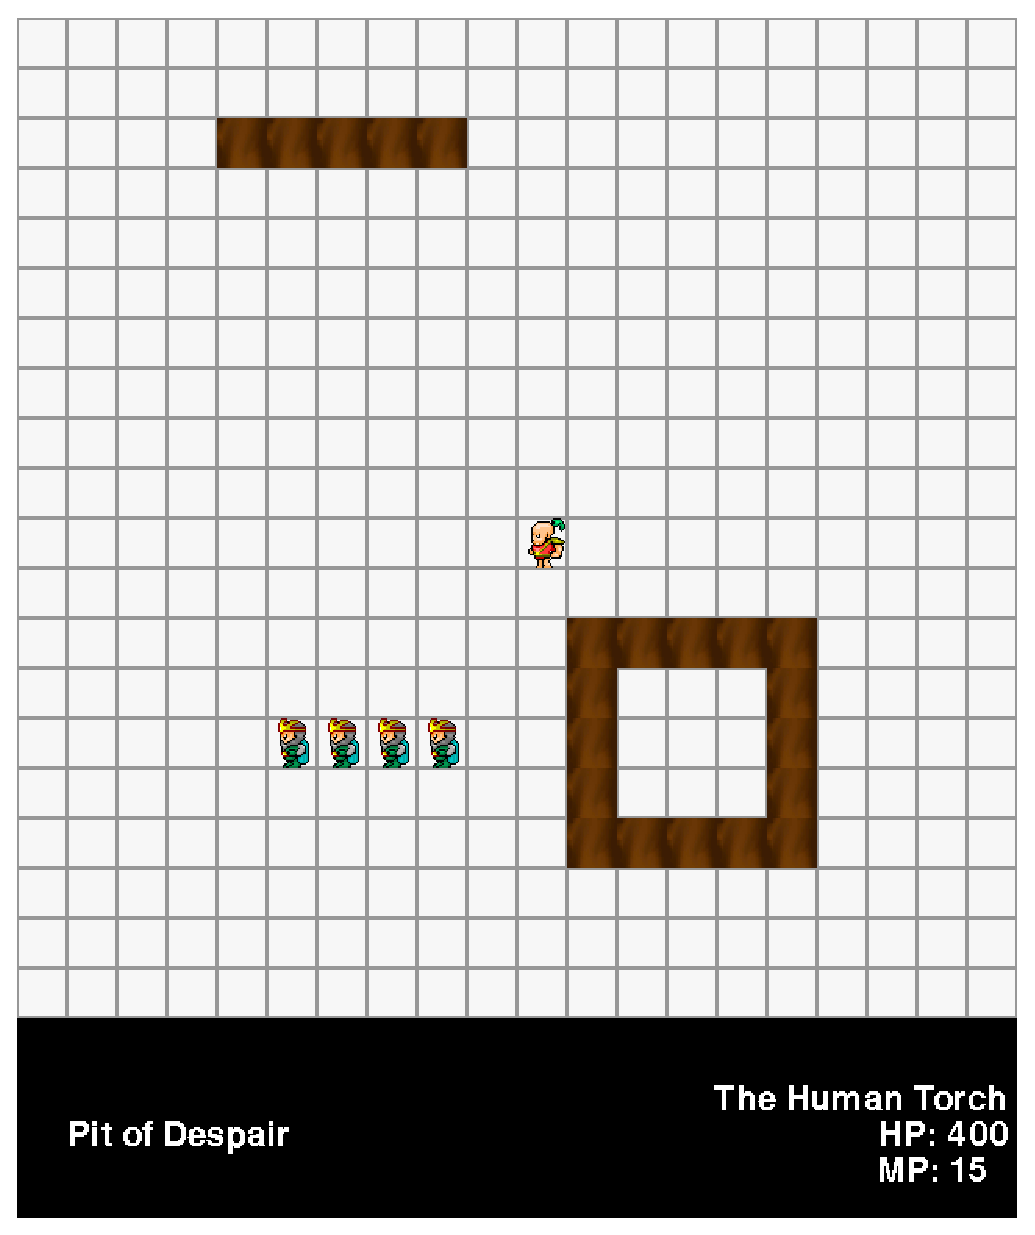
\includegraphics[width=0.8\textwidth]{images/overworld_before}
\end{center}
\caption{Overworld Screen Prior To Battle}
\end{figure}
\newpage

\begin{figure}[h!]
\begin{center}
\leavevmode
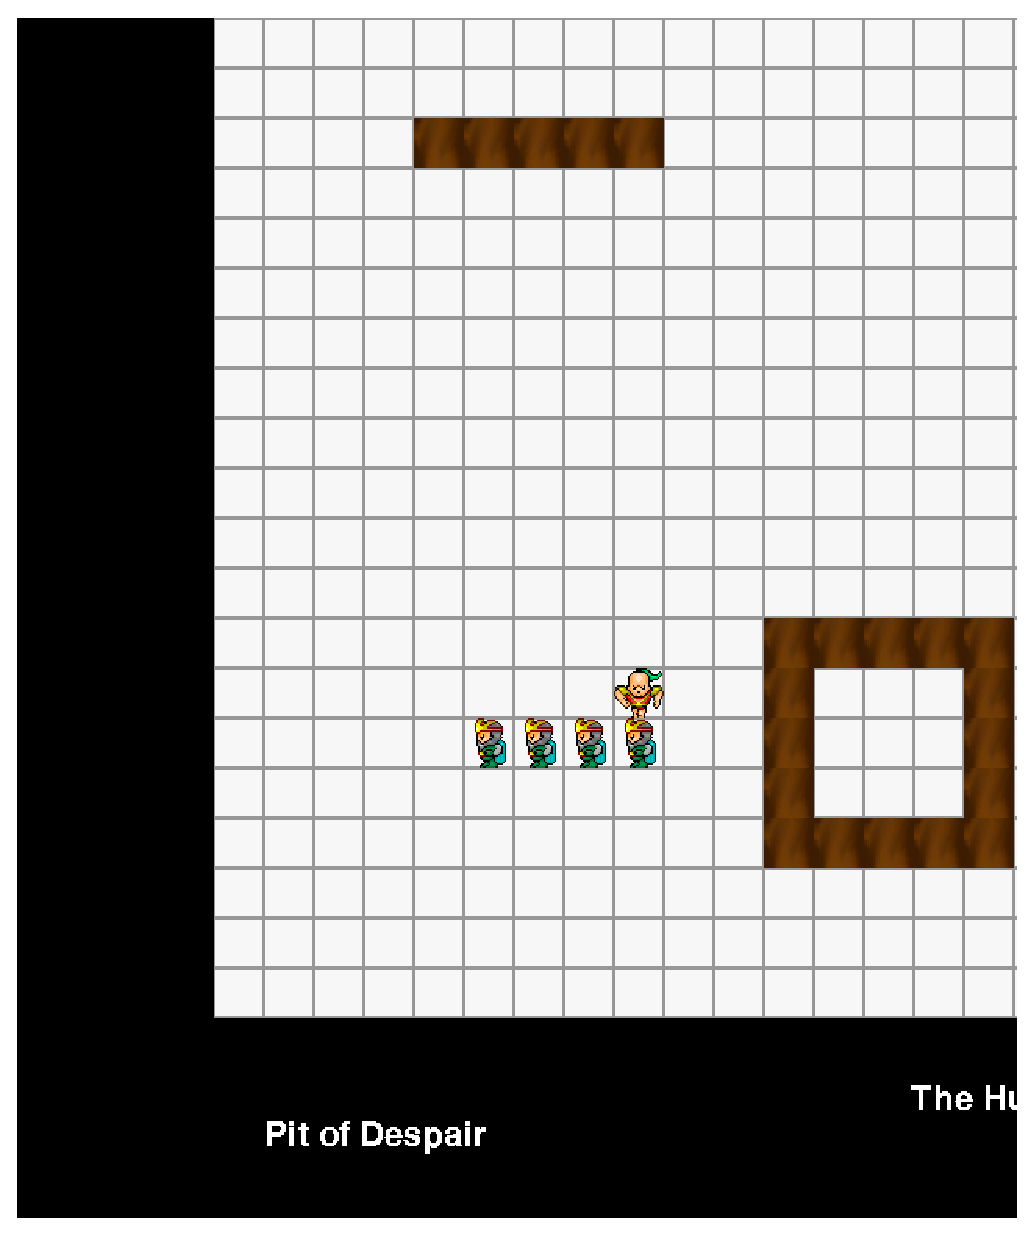
\includegraphics[width=0.8\textwidth]{images/overworld_horizlefttransition}
\end{center}
\caption{Battle Transition -- Player has collided with an NPC and screen ``slides'' to the right}
\end{figure}
\newpage

\begin{figure}[h!]
\begin{center}
\leavevmode
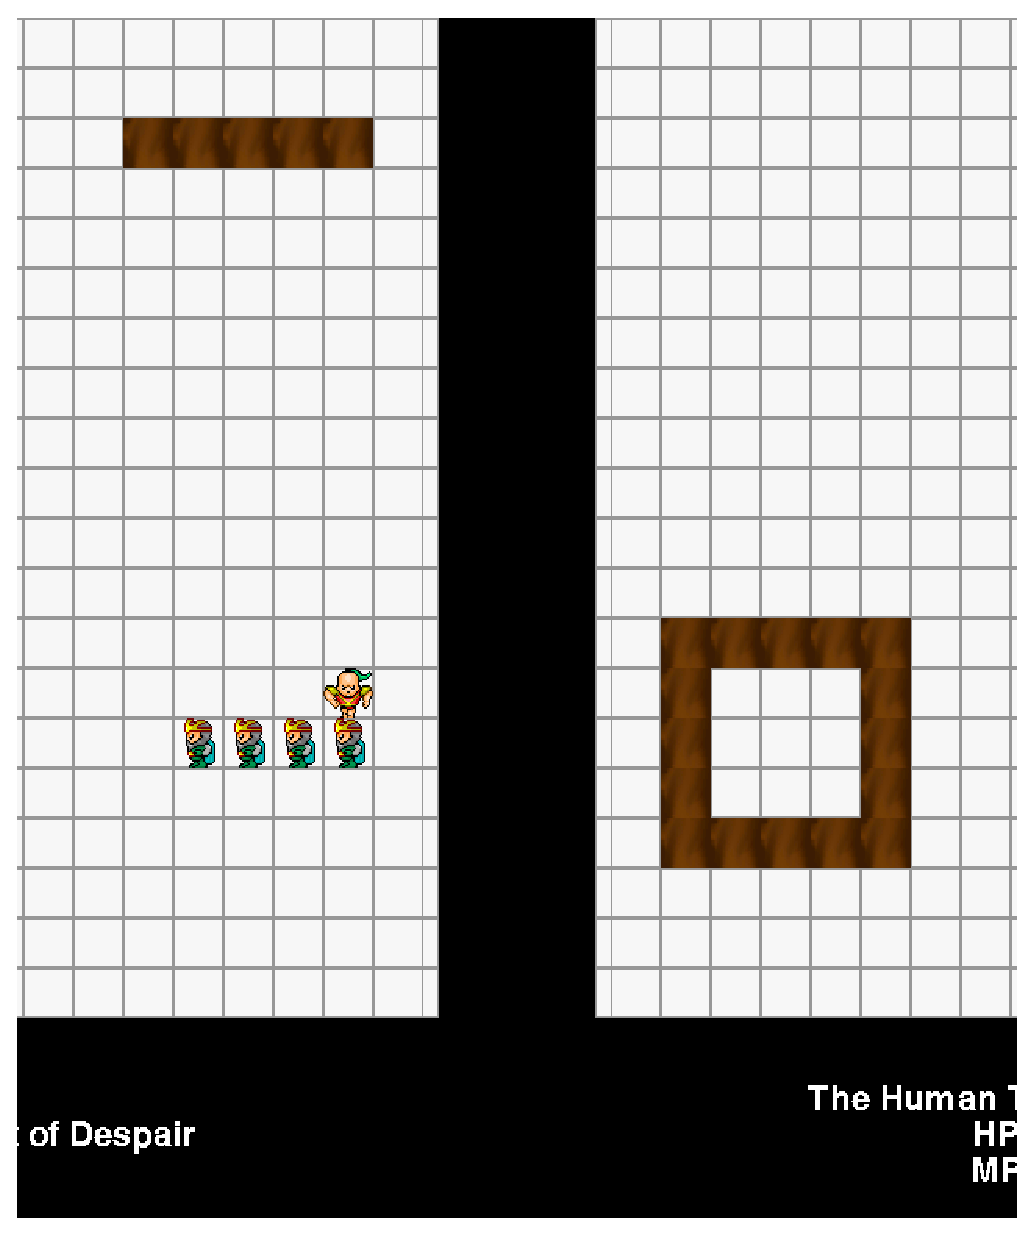
\includegraphics[width=0.8\textwidth]{images/overworld_horizsplit}
\end{center}
\caption{Battle Transition -- Alternative Transition where screen ``splits'' from the middle}
\end{figure}
\newpage

\begin{figure}[h!]
\begin{center}
\leavevmode
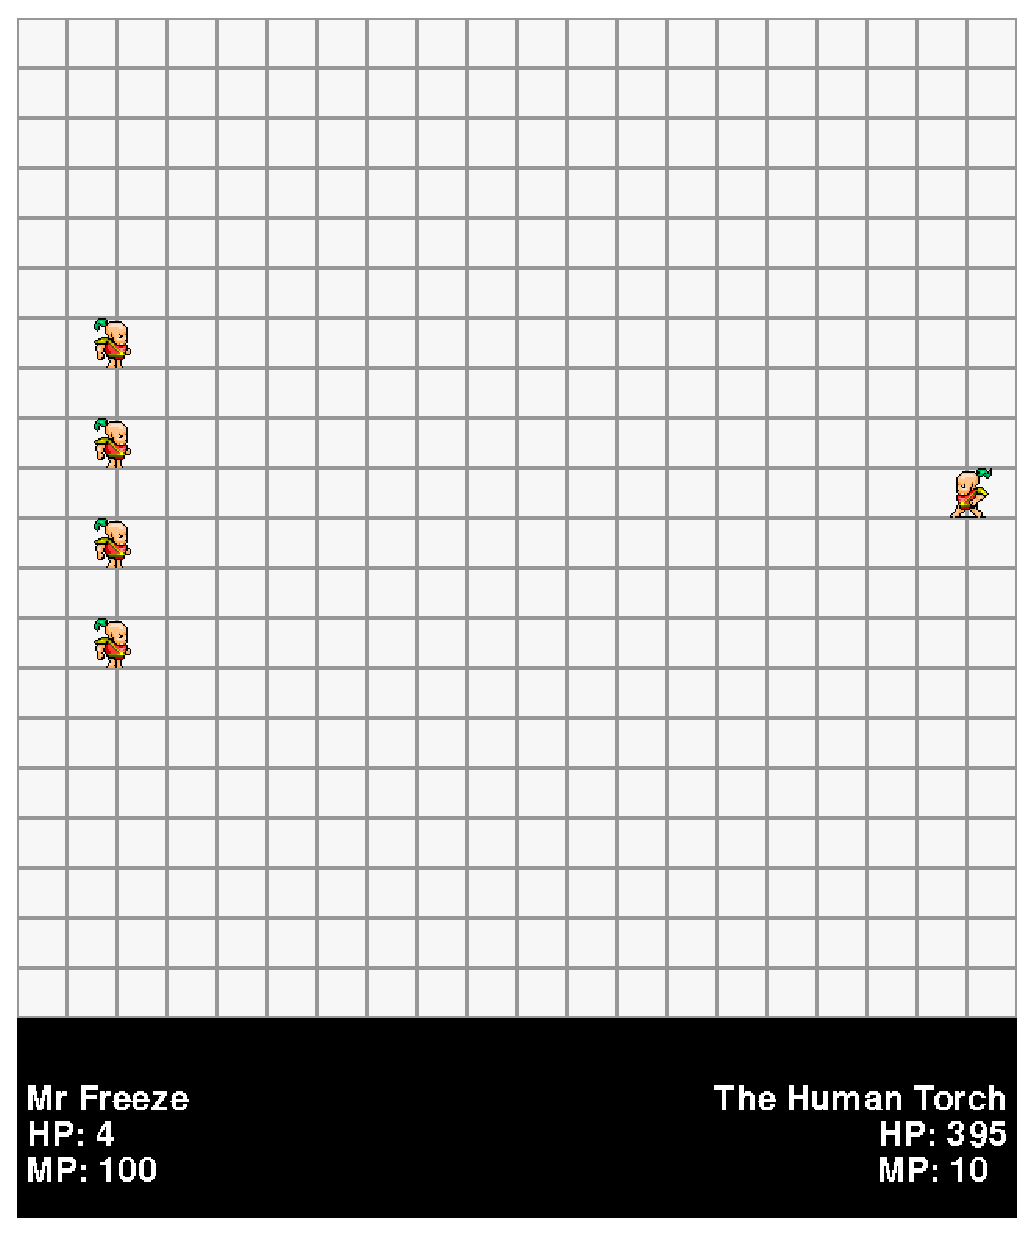
\includegraphics[width=0.8\textwidth]{images/battle_start}
\end{center}
\caption{Battle Screen -- Four enemies remain}
\end{figure}
\newpage

\begin{figure}[h!]
\begin{center}
\leavevmode
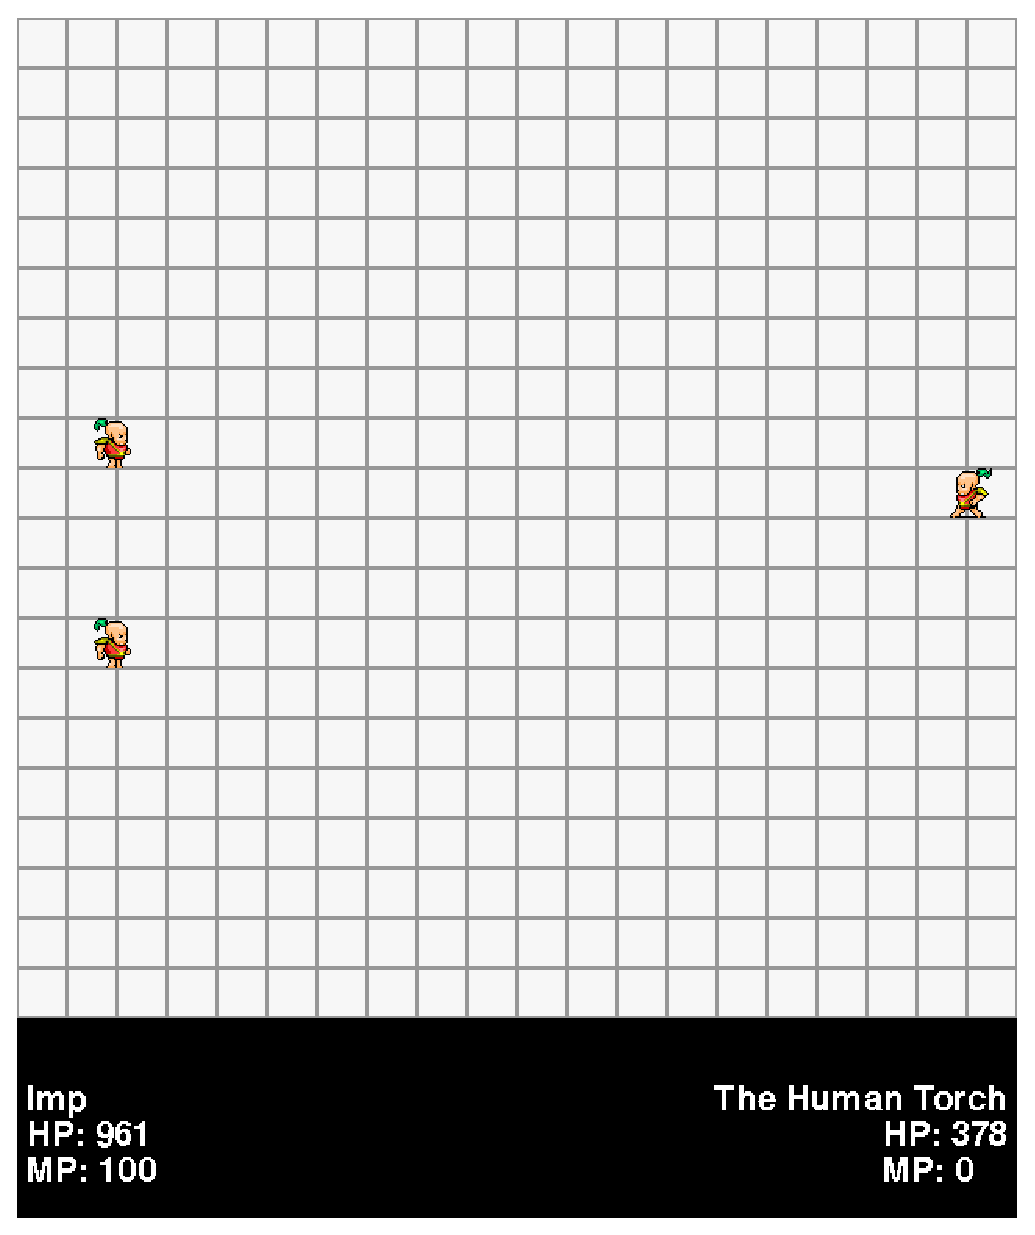
\includegraphics[width=0.8\textwidth]{images/battle_middle}
\end{center}
\caption{Battle Screen -- Two enemies remain, player has used spells and taken damage}
\end{figure}
\newpage

\begin{figure}[h!]
\begin{center}
\leavevmode
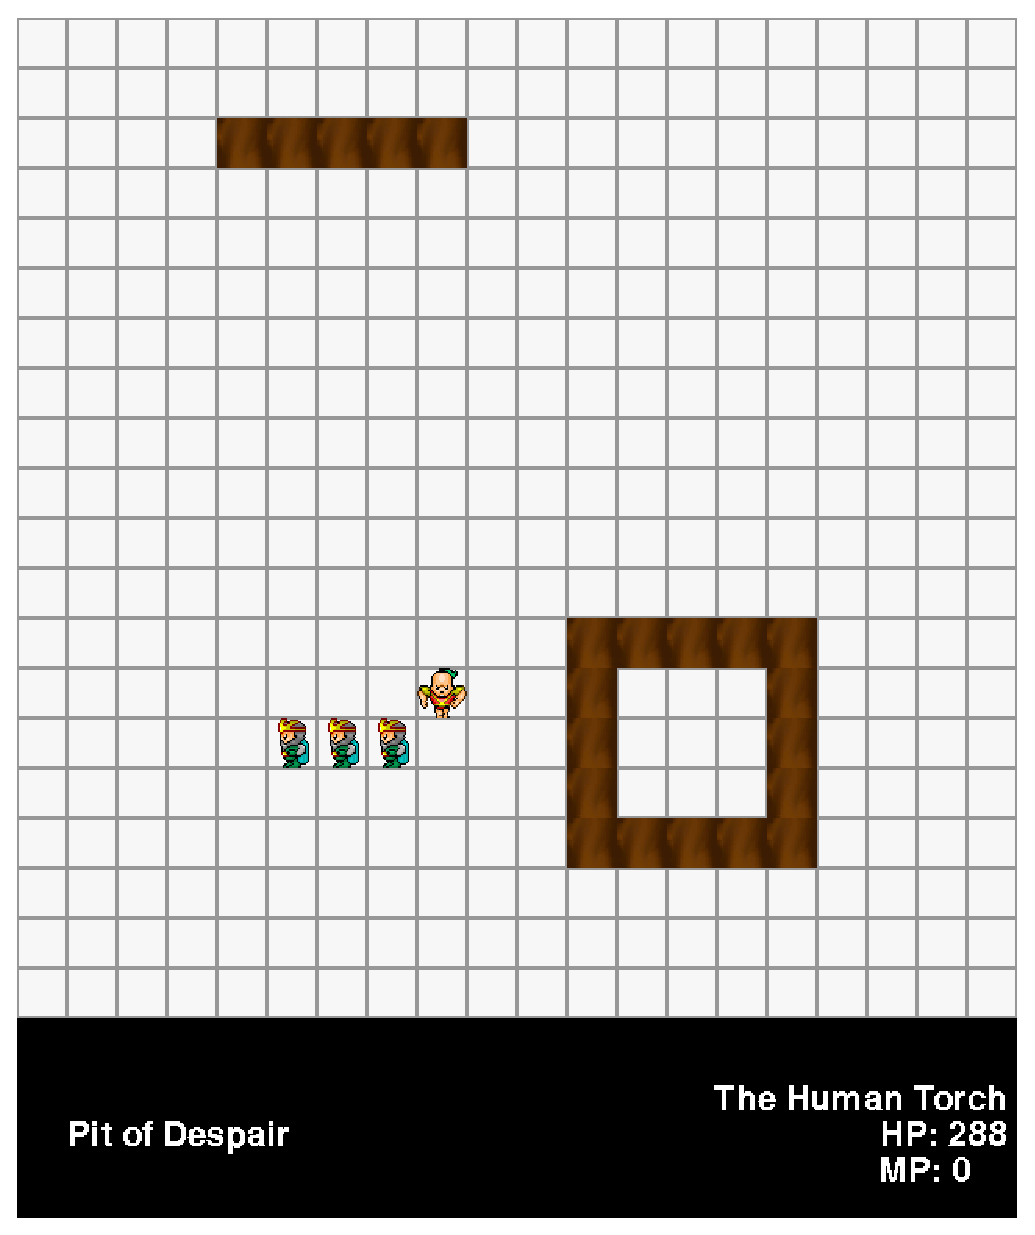
\includegraphics[width=0.8\textwidth]{images/overworld_postbattle}
\end{center}
\caption{Overworld Screen Post Battle -- Notice one of the NPC sprites has been removed and the players stats have been modified}
\end{figure}
\newpage


\section{Future Work}

Future endeavors in the direction of automated player game AI should probably be directed towards modifying existing games, rather than continuing work on a from-scratch game.  The bulk of development time on this project was spent developing the ``simple'' front-end and other GUI elements, rather than fleshing out the backend battle system.  If an existing RPG were used instead of starting from scratch more time could have been spent on adding more complicated Conditions, Actions, and Strategies.  Most RPG type games probably feature a very structured set of actions and character interactions.  Adding on a structured stimuli-response system similar to what has been prototyped here would be a relatively simple task.

Once the backend has been put in place, competitions could be formed around the system, such as those often associated with RoboCode.  Player vs Player would be tricky to set up.  Player vs. Computer situations would be much easier to establish and regulate.  Categories such as least moves to win against pregenerated opponents would have people optimizing their strategies well. 

If the prototype implementation were to be improved in some manner, the best way forward would be to make the combat more complex so that more complex strategies could be built around it.  Ideas for expansion would involve multiple characters on the player team, the ability to target multiple combatants with abilities, and strategies that can choose targets based on these additions. More complex equipment loadouts and damage potential could also lead to to more complex strategy possibilities.

\section{Appendices}

The source code for this project is available on GitHub, located at \url{https://github.com/mgius/senior_project}, under a BSD license.  Media assets are licensed Creative Commons Attribution NonCommercial.

%(as needed) for proofs, user manuals, etc.

%Please remember that this is a formal report that will remain in the library after you graduate. As such, it should be written with formal language and clear exposition. This report should demonstrate your mastery of the topic you have chosen for your senior project. It should be something you are proud of in the end.

\newpage

\bibliographystyle{plain}
\bibliography{labreport}

\end{document}
